\documentclass[12pt]{report}
\hbadness=100000%
\usepackage[margin=1in]{geometry}
\setlength{\parskip}{5pt}
\usepackage{xurl}
\usepackage{amsmath}
\usepackage{mathtools}
\usepackage{graphicx}
\usepackage{float}
\usepackage{textcomp}
\usepackage{gensymb}
\renewcommand{\bibname}{References}


\title{ECE 496 - Silicon Integrated Circuit Design Technology  Lab 2: Silicon Wafer Cleaning \\ Spring 2026, Lab Section B}
\author{Gianni Avilan-Losee}
\date{\today}
\begin{document}
\maketitle
\setcounter{chapter}{2}
\setcounter{section}{0}
\section{Objectives}

This lab's objective was to familiarize ourselves with the industry-standard process for silicon wafer cleaning, a vital first step in the silicon integrated circuit fabrication workflow. Understanding the cleaning process ensures that there are as few contaminants as possible present on the wafer prior to oxidation, reducing quality issues and other complications down the line.

\section{Background}

\subsection{Microscopy and wafer inspection}

Inspection of the wafer before and after cleaning is a critical quality control measure, and in this lab, a microscope was used at 5x magnification, with the resulting image displayed on a nearby computer screen. The available microscope had the capability to switch between bright-field (BF) and dark-field (DF) microscopy modes, as well as stage control knobs to make fine adjustments in the position of the silicon wafer being viewed. 

BF microscopy illuminates the subject (in this case, the silicon wafer) against a bright background, while DF microscopy illuminates the subject against a dark background. Since the bandgap energy of pure silicon is approximately \(1.12 \ \mathrm{eV}\) at room temperature, visible light in the \(400-700 \ \mathrm{nm}\) wavelength (\(1.63-3.26 \ \mathrm{eV})\) is "absorbed" by the pure silicon, meaning that defects and very small particles present on the surface of the wafer will stand out against the dark surface of the silicon under a microscope. DF microscopy is ideal for very sensitive detection of particles and defects, while BF microscopy is more suited to a general, first-pass inspection of the wafer. Experimental results from our inspections in the lab may be found in the following sections. As discussed in \cite{inspection}, defect inspection techniques are an ongoing area of research, of particular importance as process size becomes smaller and smaller over time; techniques such as scanning electron microscopy (SEM) and e-beam inspection may be relevant to more advanced processes than the one carried out in this lab.

\subsection{Wafer cleaning}

The industry standard for wafer cleaning is almost exclusively based on the principles of the RCA clean, a process developed by Werner Kern in 1965 \cite{kern}.

A modified version of the RCA clean is used for this lab, substituting sulfuric acid for hydrochloric acid, presumably for safety reasons. The two solutions used in the RCA clean, SC-1 and SC-2, are prepared as follows for our lab: 

\textbf{SC-1:}
\begin{itemize}
	\item 5 parts deionized water \((H_2O)\).
	\item 1 part ammonium hydroxide \((NH_4OH)\).
	\item 1 part hydrogen peroxide \(H_2O_2\).
\end{itemize}

\textbf{SC-2}
\begin{itemize}
	\item 6 parts deionized water \((H_2O)\).
	\item 1 part sulfuric acid \((H_2SO_4)\).
	\item 1 part hydrogen peroxide \((H_2O_2)\).
\end{itemize}

\subsection{Wafer drying}

To dry cleaned wafers, a Verteq Superclean spin rinse dryer was used, which spins the cleaned wafers at high speed while rinsing them with deionized water, and then continues spinning them while blowing any remaining liquid off the surface using pure nitrogen gas. Spin drying is one of the standard techniques used in industry, among others \cite{drying}.

\section{Procedure}

After following proper gowning and cleanroom procedure, and entering the lab, the 100mm wafers were subjected to a first-pass inspection using BF and DF microscopy. Larger particles such as dust and dirt detected on the surface were blown off using a pressurized nitrogen gas nozzle, at which point the wafers were returned to their carrying cases and transferred to the cleaning bay.

First, the wafers were prepared for an RCA clean by transferring them to a Teflon wafer boat, with a consistent orientation. Then, the wafers were lowered into a tub filled with SC-1, held at \(60 \degree \mathrm{C}\), and slowly agitated for 10 minutes before being slowly removed and allowed to drip dry for 30-60 seconds over the SC-1 tub. Then, the wafer carries was placed inside the cascade rinse tank, sprayed with deionized water, and then submerged briefly. The cascade rinse tank then auto-drained and sprayed the wafers once again. The wafers were blown with pressurized nitrogen gas to dry them somewhat, and then transferred to individual wafer trays for the SC-2 step (this was done due to space considerations, and a smaller amount of SC-2 available versus SC-1.)

Then, the wafers were submerged in SC-2 and agitated slowly for another period of 10 minutes. This was followed by a second cycle in the cascade rinse tank, identical to the previous cycle.

Then, the wafers were rolled into a second processing boat, which was inserted into the Verteq spin rinse dryer, which was set to autocycle for a period of 10 minutes (5 minutes of rinsing time, and 5 minutes of drying time).

The wafers were then transferred back to their carrying cases and returned to the inspection bay, where they were inspected once again using DF microscopy to ensure that all impurities and foreign particles were removed by the RCA cleaning process.

\section{Results and Discussion}
\subsection{Initial wafer inspection}
In the initial inspection, BF and DF microscopy revealed a number of small, foreign particles on the wafer's surface, likely dust or other impurities (see Figs. 2.1, 2.2).

\begin{figure}[H]
  \centering
  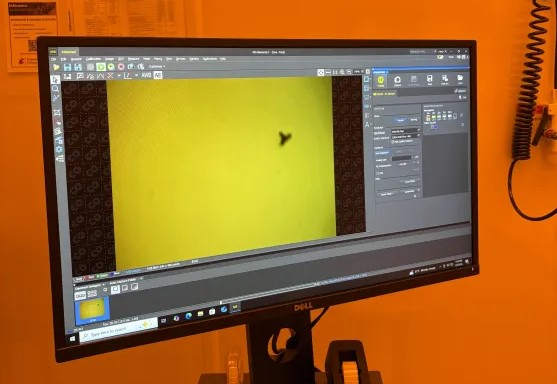
\includegraphics[width=0.8\textwidth]{lab-report-1_fig-1.jpg}
  \caption{Initial inspection under BF microscopy}
  \label{fig:initial_1}
\end{figure}
\begin{figure}[H]
  \centering
  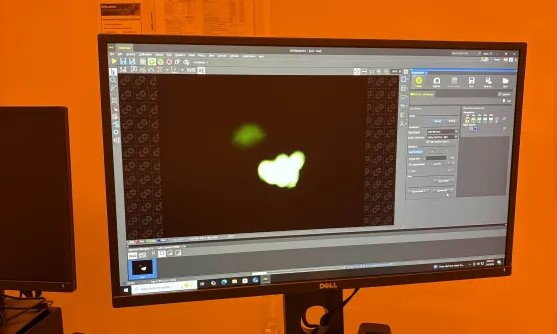
\includegraphics[width=0.8\textwidth]{lab-report-1_fig-2.jpg}
  \caption{Initial inspection under DF microscopy}
  \label{fig:initial_2}
\end{figure}

The above procedure was followed for the RCA clean, as shown in Figs. 2.3, 2.4, as well as the spin rinse dry, as described, as shown in Fig. 2.5, with no notable issues or changes. 

\begin{figure}[H]
  \centering
  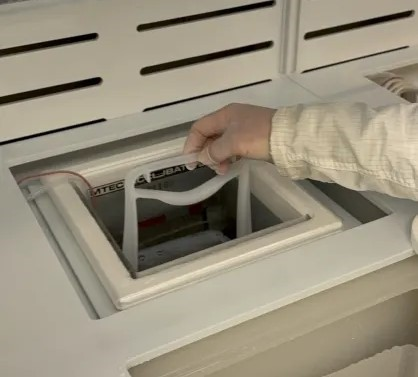
\includegraphics[width=0.8\textwidth]{lab-report-1_fig-3.jpg}
  \caption{Submersion in SC-1}
  \label{fig:sub}
\end{figure}

\begin{figure}[H]
  \centering
  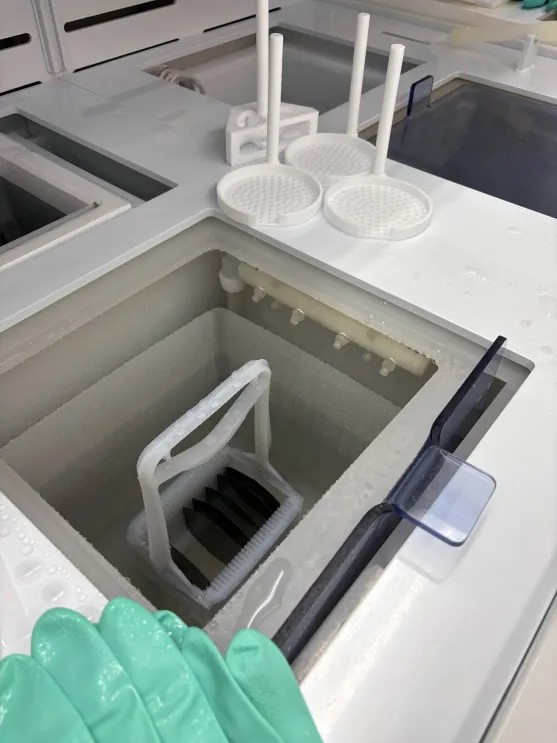
\includegraphics[width=0.8\textwidth]{lab-report-1_fig-4.jpg}
  \caption{Cascade rinse with DI}
  \label{fig:rinse}
\end{figure}

\begin{figure}[H]
  \centering
  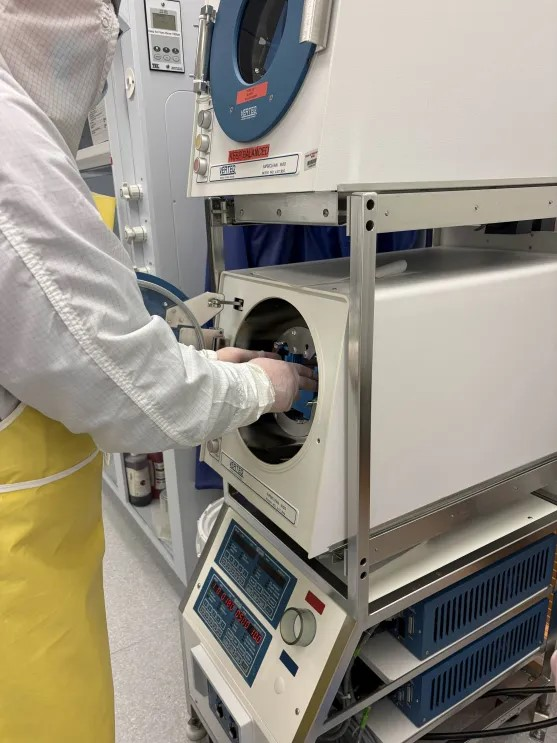
\includegraphics[width=0.8\textwidth]{lab-report-1_fig-5.jpg}
  \caption{Spin rinse and dry}
  \label{fig:spin}
\end{figure}

We may note that upon submerging the wafers in SC-1, the mixture bubbled slightly for several seconds, implying that there were a significant number of impurities present on the surface of the wafer which were initially dissolved in the SC-1.

Finally, once the RCA clean and spin rinse/dry steps were complete, the wafer was inspected to ensure that no impurities remained on the surface. As shown in Fig. 2.6, DF microscopy revealed no impurities, and the microscope stage was moved so as to inspect the entire surface of the wafer, within reasonable time constraints.

\begin{figure}[H]
  \centering
  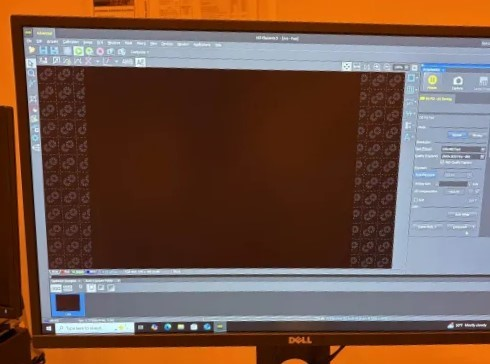
\includegraphics[width=0.8\textwidth]{lab-report-1_fig-6.jpg}
  \caption{Final inspection under DF microscopy}
  \label{fig:label}
\end{figure}

\section{Conclusion}

In conclusion, the above process clarified both the importance and effectiveness of the RCA clean for a successful semiconductor manufacturing workflow. Though an RCA clean as an intermediate step between all other manufacturing steps would be ideal, it is especially critical prior to oxidation, which will be the next step in our lab procedure. Post-cleaning inspection of the wafer, as shown in the Results and Discussion section, shows that the RCA clean is effective at removing impurities and particles from the surface of the silicon wafer, at least at the 5x magnification level. More sophisticated inspection methods may have revealed leftover impurities or defects that will affect the final product; however, for our purposes, the above RCA process was sufficient to move forward with oxidation.

\begin{thebibliography}{4}
	\bibitem{inspection} Ralf Buengener "Defect inspection strategies for 14 nm semiconductor technology", Proc. SPIE 8466, Instrumentation, Metrology, and Standards for Nanomanufacturing, Optics, and Semiconductors VI, 846607 (11 October 2012); https://doi.org/10.1117/12.928664.
	\bibitem{kern} Werner, Kern "The Evolution of Silicon Wafer Cleaning Technology", J. Electrochem. Soc. 137 1887, 1990. 
	\bibitem{drying}Wim Fyen, Frank Holsteyns, Twan Bearda, Sophia Arnauts, Jan Van Steenbergen, Geert Doumen, Karine Kenis, Paul W. Mertens,
Chapter 19 - A Detailed Study of Semiconductor Wafer Drying,
Editor(s): Rajiv Kohli, K.L. Mittal,
Developments in Surface Contamination and Cleaning (Second Edition),
William Andrew Publishing,
2008,
Pages 795-854,
ISBN 9780323299602,
https://doi.org/10.1016/B978-0-323-29960-2.00019-8.
\end{thebibliography}

\end{document}

